\subsection{Tarefa 1 -- Exploração de Funções de Ativação}

\begin{comandoquestao}
   Nesta tarefa, você explorará o impacto de diferentes funções de ativação no desempenho da rede neural. A função de ativação controla como os neurônios transformam os dados de entrada, e diferentes funções podem influenciar a capacidade de aprendizado da rede.
\end{comandoquestao}

A rede neural dada como exemplo utiliza a função Gelu como função de ativação nas camadas intermediárias. Vericamos o comportamento do erro de treinamento em relação ao número de épocas de treinamento (figura \ref{tarefa01:gelu:treinamento}), bem como a comparação dos dados previstos pela rede dados em relação aos dados de treinamento na figura \ref{tarefa01:gelu:predicoes}.

\begin{figure}[htb]
	\centering
	\begin{minipage}{0.45\textwidth}
	\centering
	\caption{Gelu: Treinamento} \label{tarefa01:gelu:treinamento}
	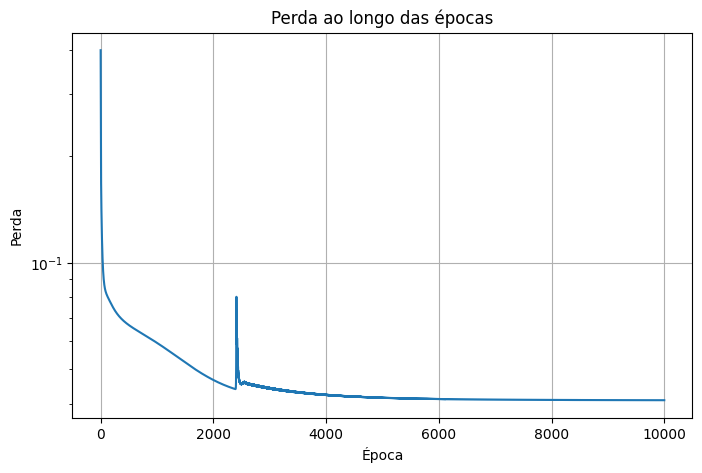
\includegraphics[width=\textwidth]{./0803_imgs/png-241111-212601400-7995113924505873963.png}
	%\legend{Fonte: Gerado peloComando da atividade}
	\end{minipage}
	\hfill
	\begin{minipage}{0.45\textwidth}
	\centering
	\caption{Gelu: predições} \label{tarefa01:gelu:predicoes}
	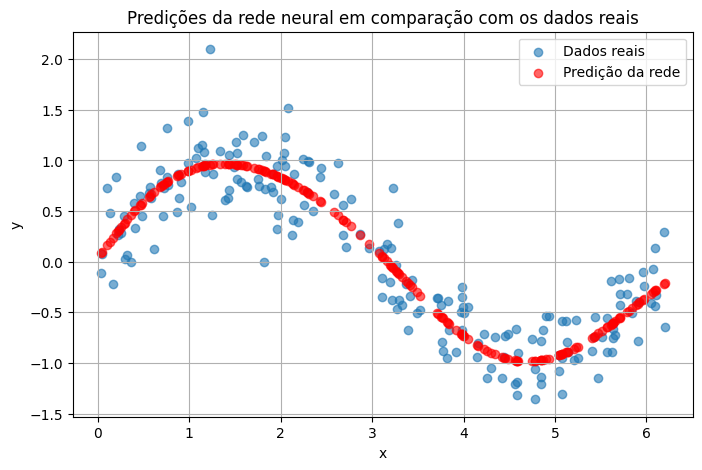
\includegraphics[width=\textwidth]{./0803_imgs/png-241111-212606975-12044568718402292765.png}
	%\legend{Fonte: \citeonline[p. 24]{araujo2012}}
	\end{minipage}
\end{figure}

Para a presente tarefa modificamos a função de ativação das camadas intermediárias para sigmóide, obtendo os resultados mostrados nas figuras \ref{tarefa01:sigmoide:treinamento} e \ref{tarefa01:simoide:predicoes}. Observamos que a com a função sigmóide ($\sigma(\cdot)$)a rede não é capaz de acompanhar as não linearidades inerentes a função seno de maneira tão precisa quando a Gelu.


\begin{figure}[htb]
	\centering
	\begin{minipage}{0.45\textwidth}
	\centering
	\caption{Sigmóide: Treinamento} \label{tarefa01:sigmoide:treinamento}
	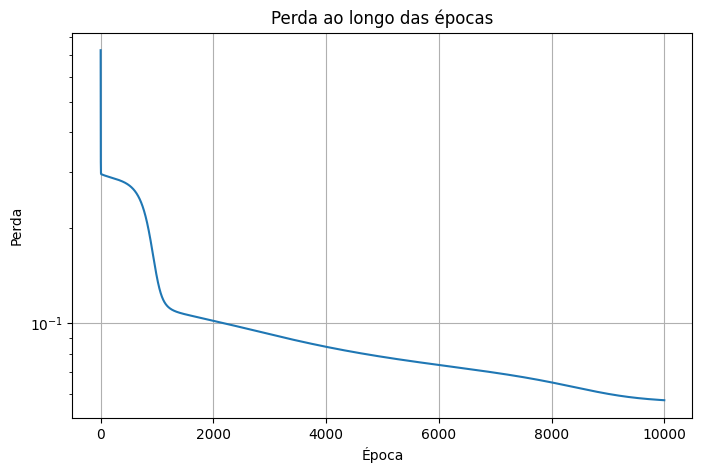
\includegraphics[width=\textwidth]{./0803_imgs/png-241110-142600634-18420033062344975583.png}
	%\legend{Fonte: Gerado peloComando da atividade}
	\end{minipage}
	\hfill
	\begin{minipage}{0.45\textwidth}
	\centering
	\caption{Sigmóide: predições} \label{tarefa01:simoide:predicoes}
	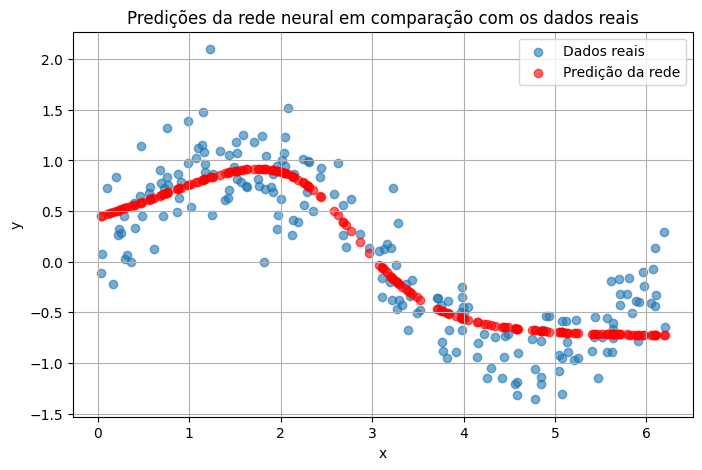
\includegraphics[width=\textwidth]{./0803_imgs/png-241110-143132585-16405151944787820073.png}
	%\legend{Fonte: \citeonline[p. 24]{araujo2012}}
	\end{minipage}
\end{figure}

Em uma segundo etapa, a função de ativação das camadas intermediárias foi modificada para a função Relu. Obtivemos os seguintes resultados da evolução das perdas durante o treinamento e do teste de predição da rede neural treinada mostrados nas \cref{tarefa01:relu:treinamento,tarefa01:relu:predicoes}. Observamos que com essa função de ativação obtivemos o gráfico de perda ao longo das épocas mais ruidoso. O que pode indicar uma inicialização de parâmetros e/ou taxa de aprendizada que pode ser melhorada para este tipo de rede neural. Em especial a inicialização do \emph{bias} requer uma atenção especial nesse caso, visto que para a função Relu é adequado um bias maior que 0.

Outro ponto interessante que pode ser observado no predição da rede neural é que o modelo treinado não parece replicar uma curva continuamente diferenciável, mas tenta replicar a senóide através de trechos de funções afins. Essa observação vai ao encontro da característica da função Relu a qual não é continuamente diferenciável.

\begin{figure}[htb]
	\centering
	\begin{minipage}{0.45\textwidth}
	\centering
	\caption{Relu: Treinamento} \label{tarefa01:relu:treinamento}
	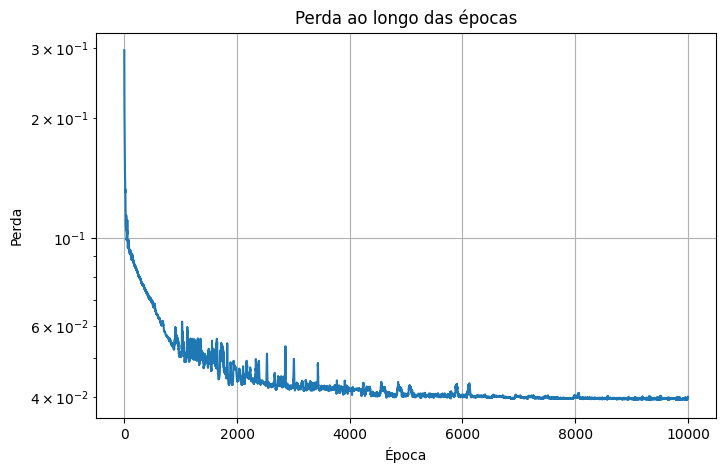
\includegraphics[width=\textwidth]{./0803_imgs/png-241110-145116395-16963719957492600077.png}
	%\legend{Fonte: Gerado peloComando da atividade}
	\end{minipage}
	\hfill
	\begin{minipage}{0.45\textwidth}
	\centering
	\caption{Relu: predições} \label{tarefa01:relu:predicoes}
	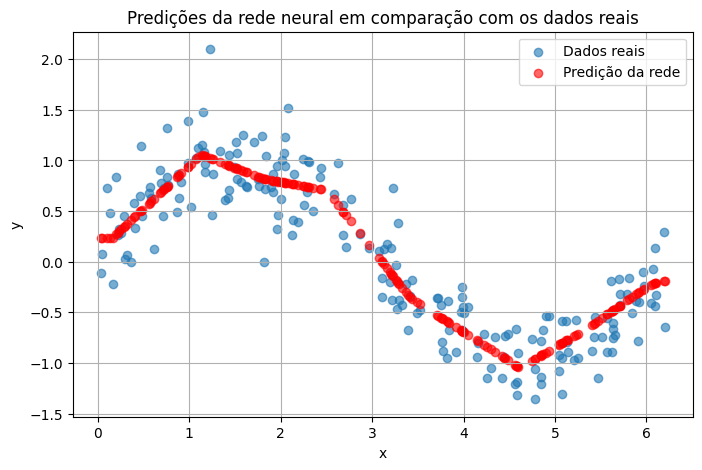
\includegraphics[width=\textwidth]{./0803_imgs/png-241111-212509484-7783840008639668300.png}
	%\legend{Fonte: \citeonline[p. 24]{araujo2012}}
	\end{minipage}
\end{figure}

Por fim, comparamos na \cref{tarefa01:tab:funcoes} os erros de treinamento para a época 9900 de cada uma das redes neurais com diferentes funções de ativação.

\begin{table}[htb]
	\centering
	\caption{Comparação das perdas de treinamento}
	\label{tarefa01:tab:funcoes}
	\begin{tabular}{ l | c | c }
		função & época & perda \\
		\hline
		Gelu & 9900 &  0.04087 \\
		Sigmóide & 9900 & 0.05731 \\
		Relu & 9900 & 0.03939 \\
	\end{tabular}
\end{table}
